\documentclass[11pt,spanish,a4paper,]{article}
\usepackage{lmodern}
%\usepackage[spanish]{babel} %walter
\usepackage{amssymb,amsmath}
\usepackage{ifxetex,ifluatex}
\usepackage{fixltx2e} % provides \textsubscript
\ifnum 0\ifxetex 1\fi\ifluatex 1\fi=0 % if pdftex
  \usepackage[T1]{fontenc}
  \usepackage[utf8]{inputenc}
\else % if luatex or xelatex
  \usepackage{unicode-math}
  \defaultfontfeatures{Ligatures=TeX,Scale=MatchLowercase}
\fi
% use upquote if available, for straight quotes in verbatim environments
\IfFileExists{upquote.sty}{\usepackage{upquote}}{}
% use microtype if available
\IfFileExists{microtype.sty}{%
\usepackage[]{microtype}
\UseMicrotypeSet[protrusion]{basicmath} % disable protrusion for tt fonts
}{}
\PassOptionsToPackage{hyphens}{url} % url is loaded by hyperref
\usepackage[unicode=true]{hyperref}
\PassOptionsToPackage{usenames,dvipsnames}{color} % color is loaded by hyperref
\hypersetup{
            pdftitle={P1 - Uso de Smartphones y Riesgo de Adiccion},
            colorlinks=true,
            linkcolor=blue,
            citecolor=Blue,
            urlcolor=Blue,
            breaklinks=true}
\urlstyle{same}  % don't use monospace font for urls
\usepackage{geometry}
\geometry{a4paper, centering, text={16cm,25cm}}
\ifnum 0\ifxetex 1\fi\ifluatex 1\fi=0 % if pdftex
  \usepackage[shorthands=off,main=spanish]{babel}
\else
  \usepackage{polyglossia}
  \setmainlanguage[]{}
\fi
\usepackage[style=authoryear-comp,]{biblatex}
\addbibresource{references.bib}
\usepackage{color}
\usepackage{fancyvrb}
\newcommand{\VerbBar}{|}
\newcommand{\VERB}{\Verb[commandchars=\\\{\}]}
\DefineVerbatimEnvironment{Highlighting}{Verbatim}{commandchars=\\\{\}}
% Add ',fontsize=\small' for more characters per line
\usepackage{framed}
\definecolor{shadecolor}{RGB}{241,243,245}
\newenvironment{Shaded}{\begin{snugshade}}{\end{snugshade}}
\newcommand{\AlertTok}[1]{\textcolor[rgb]{0.68,0.00,0.00}{#1}}
\newcommand{\AnnotationTok}[1]{\textcolor[rgb]{0.37,0.37,0.37}{#1}}
\newcommand{\AttributeTok}[1]{\textcolor[rgb]{0.40,0.45,0.13}{#1}}
\newcommand{\BaseNTok}[1]{\textcolor[rgb]{0.68,0.00,0.00}{#1}}
\newcommand{\BuiltInTok}[1]{\textcolor[rgb]{0.00,0.23,0.31}{#1}}
\newcommand{\CharTok}[1]{\textcolor[rgb]{0.13,0.47,0.30}{#1}}
\newcommand{\CommentTok}[1]{\textcolor[rgb]{0.37,0.37,0.37}{#1}}
\newcommand{\CommentVarTok}[1]{\textcolor[rgb]{0.37,0.37,0.37}{\textit{#1}}}
\newcommand{\ConstantTok}[1]{\textcolor[rgb]{0.56,0.35,0.01}{#1}}
\newcommand{\ControlFlowTok}[1]{\textcolor[rgb]{0.00,0.23,0.31}{\textbf{#1}}}
\newcommand{\DataTypeTok}[1]{\textcolor[rgb]{0.68,0.00,0.00}{#1}}
\newcommand{\DecValTok}[1]{\textcolor[rgb]{0.68,0.00,0.00}{#1}}
\newcommand{\DocumentationTok}[1]{\textcolor[rgb]{0.37,0.37,0.37}{\textit{#1}}}
\newcommand{\ErrorTok}[1]{\textcolor[rgb]{0.68,0.00,0.00}{#1}}
\newcommand{\ExtensionTok}[1]{\textcolor[rgb]{0.00,0.23,0.31}{#1}}
\newcommand{\FloatTok}[1]{\textcolor[rgb]{0.68,0.00,0.00}{#1}}
\newcommand{\FunctionTok}[1]{\textcolor[rgb]{0.28,0.35,0.67}{#1}}
\newcommand{\ImportTok}[1]{\textcolor[rgb]{0.00,0.46,0.62}{#1}}
\newcommand{\InformationTok}[1]{\textcolor[rgb]{0.37,0.37,0.37}{#1}}
\newcommand{\KeywordTok}[1]{\textcolor[rgb]{0.00,0.23,0.31}{\textbf{#1}}}
\newcommand{\NormalTok}[1]{\textcolor[rgb]{0.00,0.23,0.31}{#1}}
\newcommand{\OperatorTok}[1]{\textcolor[rgb]{0.37,0.37,0.37}{#1}}
\newcommand{\OtherTok}[1]{\textcolor[rgb]{0.00,0.23,0.31}{#1}}
\newcommand{\PreprocessorTok}[1]{\textcolor[rgb]{0.68,0.00,0.00}{#1}}
\newcommand{\RegionMarkerTok}[1]{\textcolor[rgb]{0.00,0.23,0.31}{#1}}
\newcommand{\SpecialCharTok}[1]{\textcolor[rgb]{0.37,0.37,0.37}{#1}}
\newcommand{\SpecialStringTok}[1]{\textcolor[rgb]{0.13,0.47,0.30}{#1}}
\newcommand{\StringTok}[1]{\textcolor[rgb]{0.13,0.47,0.30}{#1}}
\newcommand{\VariableTok}[1]{\textcolor[rgb]{0.07,0.07,0.07}{#1}}
\newcommand{\VerbatimStringTok}[1]{\textcolor[rgb]{0.13,0.47,0.30}{#1}}
\newcommand{\WarningTok}[1]{\textcolor[rgb]{0.37,0.37,0.37}{\textit{#1}}}
\usepackage{longtable,booktabs}
% Fix footnotes in tables (requires footnote package)
\IfFileExists{footnote.sty}{\usepackage{footnote}\makesavenoteenv{long table}}{}
\usepackage{graphicx,grffile}
\makeatletter
\def\maxwidth{\ifdim\Gin@nat@width>\linewidth\linewidth\else\Gin@nat@width\fi}
\def\maxheight{\ifdim\Gin@nat@height>\textheight\textheight\else\Gin@nat@height\fi}
\makeatother
% Scale images if necessary, so that they will not overflow the page
% margins by default, and it is still possible to overwrite the defaults
% using explicit options in \includegraphics[width, height, ...]{}
\setkeys{Gin}{width=\maxwidth,height=\maxheight,keepaspectratio}
\IfFileExists{parskip.sty}{%
\usepackage{parskip}
}{% else
\setlength{\parindent}{0pt}
\setlength{\parskip}{6pt plus 2pt minus 1pt}
}
\setlength{\emergencystretch}{3em}  % prevent overfull lines
\providecommand{\tightlist}{%
  \setlength{\itemsep}{0pt}\setlength{\parskip}{0pt}}
\setcounter{secnumdepth}{5}

% set default figure placement to htbp
\makeatletter
\def\fps@figure{htbp}
\makeatother


\title{P1 - Uso de Smartphones y Riesgo de Adiccion}

%% MONASH STUFF

%% CAPTIONS
\RequirePackage{caption}
\DeclareCaptionStyle{italic}[justification=centering]
 {labelfont={bf},textfont={it},labelsep=colon}
\captionsetup[figure]{style=italic,format=hang,singlelinecheck=true}
\captionsetup[table]{style=italic,format=hang,singlelinecheck=true}
%% FONT
\usepackage{bera}
\usepackage[charter,expert]{mathdesign}
\usepackage[lf,t]{FiraSans}
\usepackage[scale=0.9]{sourcecodepro}
\RequirePackage{fontawesome}

%% HEADERS AND FOOTERS
\RequirePackage{fancyhdr}
\pagestyle{fancy}
\rfoot{\Large\sffamily\raisebox{-0.1cm}{\textbf{\thepage}}}
\makeatletter
\lhead{\textsf{\expandafter{\@title}}}
\makeatother
\rhead{}
\cfoot{}
\setlength{\headheight}{15pt}
\renewcommand{\headrulewidth}{0.4pt}
\renewcommand{\footrulewidth}{0.4pt}
\fancypagestyle{plain}{%
\fancyhf{} % clear all header and footer fields
\fancyfoot[C]{\sffamily\thepage} % except the center
\renewcommand{\headrulewidth}{0pt}
\renewcommand{\footrulewidth}{0pt}}

%% MATHS
\RequirePackage{bm,amsmath}
\allowdisplaybreaks

%% GRAPHICS
\RequirePackage{graphicx}
\setcounter{topnumber}{2}
\setcounter{bottomnumber}{2}
\setcounter{totalnumber}{4}
\renewcommand{\topfraction}{0.85}
\renewcommand{\bottomfraction}{0.85}
\renewcommand{\textfraction}{0.15}
\renewcommand{\floatpagefraction}{0.8}

%% SECTION TITLES
\RequirePackage[compact,sf,bf]{titlesec}
\titleformat*{\section}{\Large\sf\bfseries\color[rgb]{0.0, 0.7451, 0.8745}}
\titleformat*{\subsection}{\large\sf\bfseries\color[rgb]{0.0, 0, 0}}
\titleformat*{\subsubsection}{\sf\bfseries\color[rgb]{0,0,0}}
\titlespacing{\section}{0pt}{2ex}{.5ex}
\titlespacing{\subsection}{0pt}{1.5ex}{0ex}
\titlespacing{\subsubsection}{0pt}{.5ex}{0ex}


%% TITLE PAGE
\def\Date{\number\day}
\def\Month{\ifcase\month\or
 de Enero del\or de Febrero del\or de Marzo del\or de Abril del\or de Mayo del\or de Junio del\or
de Julio del\or de Agosto del\or de Septiembre del\or de Octubre del\or de Noviembre del\or de Diciembre del\fi}
\def\Year{\number\year}

%% LINE AND PAGE BREAKING
\sloppy
\clubpenalty = 10000
\widowpenalty = 10000
\brokenpenalty = 10000
\RequirePackage{microtype}

%% PARAGRAPH BREAKS
\setlength{\parskip}{1.4ex}
\setlength{\parindent}{0em}

%% HYPERLINKS
\RequirePackage{xcolor} % Needed for links
\definecolor{darkblue}{rgb}{0,0,.6}
\RequirePackage{url}

\makeatletter
\@ifpackageloaded{hyperref}{}{\RequirePackage{hyperref}}
\makeatother
\hypersetup{
     citecolor=0 0 0,
     breaklinks=true,
     bookmarksopen=true,
     bookmarksnumbered=true,
     linkcolor=darkblue,
     urlcolor=blue,
     citecolor=darkblue,
     colorlinks=true}

\usepackage[showonlyrefs]{mathtools}
\usepackage[no-weekday]{eukdate}

%% BIBLIOGRAPHY

\makeatletter
\@ifpackageloaded{biblatex}{}{\usepackage[style=authoryear-comp, backend=biber, natbib=true]{biblatex}}
\makeatother
\ExecuteBibliographyOptions{bibencoding=utf8,minnames=1,maxnames=3, maxbibnames=99,dashed=false,terseinits=true,giveninits=true,uniquename=false,uniquelist=false,doi=false, isbn=false,url=true,sortcites=false}

\DeclareFieldFormat{url}{\texttt{\url{#1}}}
\DeclareFieldFormat[article]{pages}{#1}
\DeclareFieldFormat[inproceedings]{pages}{\lowercase{pp.}#1}
\DeclareFieldFormat[incollection]{pages}{\lowercase{pp.}#1}
\DeclareFieldFormat[article]{volume}{\mkbibbold{#1}}
\DeclareFieldFormat[article]{number}{\mkbibparens{#1}}
\DeclareFieldFormat[article]{title}{\MakeCapital{#1}}
\DeclareFieldFormat[article]{url}{}
%\DeclareFieldFormat[book]{url}{}
%\DeclareFieldFormat[inbook]{url}{}
%\DeclareFieldFormat[incollection]{url}{}
%\DeclareFieldFormat[inproceedings]{url}{}
\DeclareFieldFormat[inproceedings]{title}{#1}
\DeclareFieldFormat{shorthandwidth}{#1}
%\DeclareFieldFormat{extrayear}{}
% No dot before number of articles
\usepackage{xpatch}
\xpatchbibmacro{volume+number+eid}{\setunit*{\adddot}}{}{}{}
% Remove In: for an article.
\renewbibmacro{in:}{%
  \ifentrytype{article}{}{%
  \printtext{\bibstring{in}\intitlepunct}}}

\AtEveryBibitem{\clearfield{month}}
\AtEveryCitekey{\clearfield{month}}

\makeatletter
\DeclareDelimFormat[cbx@textcite]{nameyeardelim}{\addspace}
\makeatother

\author{\sf{\Large\textbf{Hiter Frank Rubio
Peralta}\\\large Alumno\\[0.5cm]}{\Large\textbf{Jossep Jorge Froilan
Choroco Neyra}\\\large Alumno\\[0.5cm]}{\Large\textbf{Joel David De la
Cruz Cardenas}\\\large Alumno\\[0.5cm]}{\Large\textbf{Rodrigo Octavio
Lucatoni Flores Ruiz}\\\large Alumno\\[0.5cm]}{\Large\textbf{Victor
Andres Diaz Garcia}\\\large Alumno\\[0.5cm]}}

\date{Invalid Date}
\makeatletter
%\lfoot{\sf Rubio Peralta, Neyra, Cardenas, Ruiz, Garcia: \@date}
\makeatother


%%%% PAGE STYLE FOR FRONT PAGE OF REPORTS

\makeatletter
\def\organization#1{\gdef\@organization{#1}}
\def\telephone#1{\gdef\@telephone{#1}}
\def\email#1{\gdef\@email{#1}}
\makeatother
  \organization{Introduccion a Ciencia de Datos e Inteligencia
Artificial}

  \def\name{CIENCIA DE DATOS E \newline INTELIGENCIA ARTIFICIAL}

  \telephone{+51 936 603 314}

  \email{pandascore@gmail.com}

%\def\webaddress{\url{http://buseco.monash.edu/ebs/consulting/}}
%\def\abn{12 377 614 012}
\def\extraspace{\vspace*{1.1cm}}
\makeatletter
\def\contactdetails{\faicon{phone} & \@telephone \\
                    \faicon{envelope} & \@email}
\makeatother

\usepackage[absolute,overlay]{textpos}
\setlength{\TPHorizModule}{1cm}
\setlength{\TPVertModule}{1cm}

%%%% FRONT PAGE OF REPORTS

\def\reporttype{Curso:} %walter

\long\def\front#1#2#3{
\newpage
\begin{textblock}{7}(12.7,28.2)\hfill
%\includegraphics[height=0.6cm]{_extensions/numbats/report/AACSB}~~~
%\includegraphics[height=0.6cm]{_extensions/numbats/report/EQUIS}~~~
%\includegraphics[height=0.6cm]{_extensions/numbats/report/AMBA}
\end{textblock}
\begin{singlespacing}
\thispagestyle{empty}
\vspace*{-1.4cm}
\hspace*{-1.4cm}
\hbox to 16cm{
  \hbox to 6.5cm{\vbox to 14cm{\vbox to 25cm{
    
\includegraphics[width=5.4cm]{_extensions/numbats/report/logo}
    \vfill
%    \includegraphics[width=2cm]{_extensions/numbats/report/MBSportrait}
    \vspace{0.4cm}
    \par
    \parbox{6.3cm}{\raggedright
      \sf\color[rgb]{0.0, 0.7451, 0.8745}
      {\large\textbf{\name}}\par
      \vspace{.7cm}
      \tabcolsep=0.12cm\sf\small
      \begin{tabular}{@{}ll@{}}\contactdetails
      \end{tabular}
      \vspace*{0.3cm}\par
%      ABN: \abn\par
    }
  }\vss}\hss}
  \hspace*{0.2cm}
  \hbox to 1cm{\vbox to 14cm{\rule{1pt}{26.8cm}\vss}\hss\hfill}
  \hbox to 10cm{\vbox to 14cm{\vbox to 25cm{
      \vspace*{3cm}\sf\raggedright
      \parbox{10cm}{\sf\raggedright\baselineskip=1.2cm
         \fontsize{24.88}{30}\color[rgb]{0.0, 0.7451, 0.8745}\sf\textbf{#1}}
      \par
      \vfill
      \large
      \vbox{\parskip=0.8cm #2}\par
      \vspace*{2cm}\par
      \reporttype\\[0.3cm]
      \hbox{#3}%\\[2cm]\
      \vspace*{1cm}
      {\large\sf\textbf{\Date~\Month~\Year}}
   }\vss}
  }}
\end{singlespacing}
\newpage
}

\makeatletter
\def\titlepage{\front{\expandafter{\@title}}{\@author}{\@organization}}
\makeatother

\usepackage{setspace}
\setstretch{1.25}

\newcounter{none}
\usepackage{array}
\usepackage{calc}
\makeatletter
\@ifpackageloaded{caption}{}{\usepackage{caption}}
\AtBeginDocument{%
\ifdefined\contentsname
  \renewcommand*\contentsname{Tabla de contenidos}
\else
  \newcommand\contentsname{Tabla de contenidos}
\fi
\ifdefined\listfigurename
  \renewcommand*\listfigurename{Listado de Figuras}
\else
  \newcommand\listfigurename{Listado de Figuras}
\fi
\ifdefined\listtablename
  \renewcommand*\listtablename{Listado de Tablas}
\else
  \newcommand\listtablename{Listado de Tablas}
\fi
\ifdefined\figurename
  \renewcommand*\figurename{Figura}
\else
  \newcommand\figurename{Figura}
\fi
\ifdefined\tablename
  \renewcommand*\tablename{Tabla}
\else
  \newcommand\tablename{Tabla}
\fi
}
\@ifpackageloaded{float}{}{\usepackage{float}}
\floatstyle{ruled}
\@ifundefined{c@chapter}{\newfloat{codelisting}{h}{lop}}{\newfloat{codelisting}{h}{lop}[chapter]}
\floatname{codelisting}{Listado}
\newcommand*\listoflistings{\listof{codelisting}{Listado de Listados}}
\makeatother
\makeatletter
\makeatother
\makeatletter
\@ifpackageloaded{caption}{}{\usepackage{caption}}
\@ifpackageloaded{subcaption}{}{\usepackage{subcaption}}
\makeatother


\begin{document}
\titlepage

{
\hypersetup{linkcolor=black}
\setcounter{tocdepth}{2}
\tableofcontents
}
\listoftables
\listoffigures
\providecommand{\pandocbounded}[1]{#1}

\begin{Shaded}
\begin{Highlighting}[]
\BuiltInTok{print}\NormalTok{(}\StringTok{"Hello world"}\NormalTok{)}
\ImportTok{import}\NormalTok{ matplotlib.pyplot }\ImportTok{as}\NormalTok{ plt}
\ImportTok{import}\NormalTok{ seaborn }\ImportTok{as}\NormalTok{ sns}

\CommentTok{\# Datos de ejemplo}
\NormalTok{nombres }\OperatorTok{=}\NormalTok{ [}\StringTok{"Luca"}\NormalTok{, }\StringTok{"Jossep"}\NormalTok{, }\StringTok{"David"}\NormalTok{, }\StringTok{"Victor"}\NormalTok{]}
\NormalTok{cantidades }\OperatorTok{=}\NormalTok{ [}\DecValTok{3}\NormalTok{, }\DecValTok{1}\NormalTok{, }\DecValTok{4}\NormalTok{, }\DecValTok{2}\NormalTok{]}

\CommentTok{\# Estilo visual de la gráfica}
\NormalTok{sns.set\_theme(style}\OperatorTok{=}\StringTok{"whitegrid"}\NormalTok{)}
\NormalTok{plt.figure(figsize}\OperatorTok{=}\NormalTok{(}\DecValTok{7}\NormalTok{, }\DecValTok{4}\NormalTok{))}

\CommentTok{\# Creación del gráfico de barras}
\NormalTok{sns.barplot(x}\OperatorTok{=}\NormalTok{nombres, y}\OperatorTok{=}\NormalTok{cantidades, palette}\OperatorTok{=}\StringTok{"Blues\_d"}\NormalTok{, hue}\OperatorTok{=}\NormalTok{nombres, legend}\OperatorTok{=}\VariableTok{False}\NormalTok{)}

\CommentTok{\# Personalización de etiquetas y título}
\NormalTok{plt.title(}\StringTok{"Cantidad de Mascotas por Integrante"}\NormalTok{, fontsize}\OperatorTok{=}\DecValTok{12}\NormalTok{, fontweight}\OperatorTok{=}\StringTok{"bold"}\NormalTok{)}
\NormalTok{plt.xlabel(}\StringTok{"Integrantes"}\NormalTok{)}
\NormalTok{plt.ylabel(}\StringTok{"Cantidad de Mascotas"}\NormalTok{)}

\CommentTok{\# Visualización limpia}
\NormalTok{plt.tight\_layout()}
\NormalTok{plt.show()}
\end{Highlighting}
\end{Shaded}

\begin{verbatim}
Hello world
\end{verbatim}

\pandocbounded{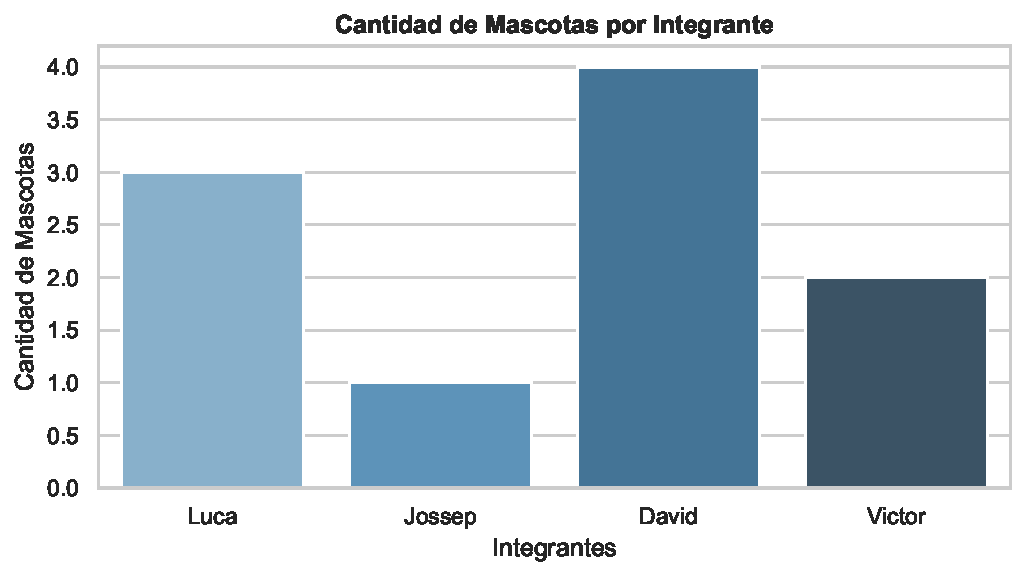
\includegraphics[keepaspectratio]{Project-Report_files/figure-pdf/cell-2-output-2.pdf}}

\newpage

\section{Resumen}\label{resumen}

\textbf{Este qmd de códex tiene los chunks de python vacíos} Este
reporte presenta la primera entrega (P1) del proyecto de Ciencia de
Datos e Inteligencia Artificial. Se explora el conjunto de datos
\textbf{Smartphone Usage and Addiction Analysis}, compuesto por 7,500
registros de uso de smartphones. El objetivo de la fase es comprender la
estructura de los datos, verificar su calidad, justificar las
transformaciones necesarias y encontrar patrones que orienten el
modelamiento de clasificación en P2.

El análisis se centra en la variable \texttt{addicted\_label}, que
distingue entre registros sin adicción (0) y con adicción (1). Los
resultados se interpretan como asociaciones observadas en el dataset; no
prueban causalidad. Esta distinción es importante porque la literatura
reporta asociaciones entre uso de smartphone y desempeño académico, pero
advierte limitaciones para atribuir causalidad \textcite{AmezBaert2020}.

\begin{Shaded}
\begin{Highlighting}[]
\ImportTok{import}\NormalTok{ pandas }\ImportTok{as}\NormalTok{ pd}

\NormalTok{data }\OperatorTok{=}\NormalTok{ \{}
    \StringTok{"names"}\NormalTok{: [}\StringTok{"Luca"}\NormalTok{, }\StringTok{"Jossep"}\NormalTok{, }\StringTok{"David"}\NormalTok{, }\StringTok{"Victor"}\NormalTok{],}
    \StringTok{"pets"}\NormalTok{: [}\StringTok{"perro"}\NormalTok{, }\StringTok{"conejo"}\NormalTok{, }\StringTok{"gato"}\NormalTok{, }\StringTok{"cuy"}\NormalTok{],}
\NormalTok{\}}

\NormalTok{df }\OperatorTok{=}\NormalTok{ pd.DataFrame(data)}
\NormalTok{df}
\end{Highlighting}
\end{Shaded}

{\def\LTcaptype{none} % do not increment counter
\begin{longtable}[]{@{}lll@{}}
\toprule\noalign{}
& names & pets \\
\midrule\noalign{}
\endhead
\bottomrule\noalign{}
\endlastfoot
0 & Luca & perro \\
1 & Jossep & conejo \\
2 & David & gato \\
3 & Victor & cuy \\
\end{longtable}
}

\section{Planteamiento del problema}\label{planteamiento-del-problema}

El uso intensivo del smartphone puede relacionarse con alteraciones del
sueño, estrés y dificultades en las actividades académicas o laborales.
La investigación sobre uso problemático del smartphone requiere
precisión conceptual: una alta frecuencia de uso no equivale
necesariamente a una condición clínica. Instrumentos de tamizaje como
SABAS permiten estudiar síntomas de uso problemático, pero no sustituyen
una evaluación profesional \textcite{Csibi2018}.

Para este proyecto, se formula la siguiente pregunta de análisis:

\begin{quote}
¿Qué patrones de uso, descanso y contexto personal están asociados con
la etiqueta de adicción en el conjunto de datos?
\end{quote}

La P1 no entrena modelos predictivos. Su finalidad es asegurar que la P2
use variables pertinentes, datos de calidad y decisiones justificadas.

\section{Contexto del dataset}\label{contexto-del-dataset}

\subsection{Fuente y unidad de
análisis}\label{fuente-y-unidad-de-anuxe1lisis}

El archivo
\texttt{Smartphone\_Usage\_And\_Addiction\_Analysis\_7500\_Rows.csv} fue
proporcionado para el proyecto y corresponde al dataset publicado como
\emph{Smartphone Usage and Addiction Analysis} en Kaggle
\textcite{KaggleDataset}. Cada fila representa a un usuario y contiene
indicadores demográficos, de comportamiento digital, descanso, estrés e
impacto percibido en actividades académicas o laborales.

La unidad de análisis es el usuario. El dataset incluye 7,500 registros
y 16 columnas originales: dos identificadores, nueve variables
numéricas, cuatro variables categóricas y la etiqueta binaria objetivo.

\subsection{Diccionario de variables}\label{diccionario-de-variables}

\begin{itemize}
\tightlist
\item
  \textbf{Identificadores:} \texttt{transaction\_id} y \texttt{user\_id}
  son variables de texto. Se usan para verificar unicidad, pero no
  aportan significado analítico y se excluirán como predictores.
\item
  \textbf{Demografía:} \texttt{age} (numérica) y \texttt{gender}
  (categórica) caracterizan la muestra.
\item
  \textbf{Uso del smartphone:} \texttt{daily\_screen\_time\_hours},
  \texttt{social\_media\_hours}, \texttt{gaming\_hours},
  \texttt{work\_study\_hours}, \texttt{notifications\_per\_day},
  \texttt{app\_opens\_per\_day} y \texttt{weekend\_screen\_time} son
  variables numéricas que miden intensidad y tipo de uso.
\item
  \textbf{Bienestar y contexto:} \texttt{sleep\_hours} es numérica;
  \texttt{stress\_level} y \texttt{academic\_work\_impact} son
  categóricas. Se emplean para explorar descanso e impacto funcional.
\item
  \textbf{Severidad:} \texttt{addiction\_level} es categórica ordinal.
  Se describe en P1, pero se excluye como predictor en P2 por fuga de
  información.
\item
  \textbf{Objetivo:} \texttt{addicted\_label} es binaria: 0 significa
  \emph{No adicción} y 1 significa \emph{Con adicción}.
\end{itemize}

La variable \texttt{addiction\_level} contiene una categorización de
severidad (\texttt{None}, \texttt{Mild}, \texttt{Moderate},
\texttt{Severe}). Por su definición operativa, puede estar construida
directamente a partir de la etiqueta final; por ello se audita
explícitamente antes de considerar su uso en P2.

\section{Carga y exploración
inicial}\label{carga-y-exploraciuxf3n-inicial}

\subsection{Dimensiones y tipos de
variables}\label{dimensiones-y-tipos-de-variables}

El dataset tiene 7,500 filas y 16 columnas originales. Las variables
numéricas se cargan como enteros o decimales; las categóricas como
texto. La estructura es consistente con un problema de clasificación
supervisada: \texttt{addicted\_label} será la etiqueta, mientras que el
resto de variables se evaluará como potencial predictor o como
identificador a excluir.

\subsection{Calidad de datos}\label{calidad-de-datos}

Se encontraron 819 valores faltantes, todos en
\texttt{addiction\_level}, y ninguna fila completamente duplicada. Una
revisión del CSV muestra que esos faltantes representan el nivel textual
\texttt{None}, es decir, ausencia de severidad registrada. No se
imputarán: \texttt{addiction\_level} se excluirá de P2 por fuga de
información. Las otras 15 columnas no tienen valores faltantes ni
requieren tratamiento de imputación. Esta decisión no implica que el
dataset esté libre de otros riesgos: se revisan también los
identificadores, rangos de las variables y la posible fuga de
información.

Los rangos son plausibles para la descripción proporcionada: edades
entre 18 y 35 años; tiempo diario de pantalla entre 3 y 12 horas; y
sueño entre 4.5 y 9 horas. Los identificadores \texttt{transaction\_id}
y \texttt{user\_id} son únicos y no representan características del
comportamiento del usuario. Se conservarán solo como trazabilidad y se
excluirán del conjunto de predictores en P2.

\section{Preprocesamiento y decisiones de data
wrangling}\label{preprocesamiento-y-decisiones-de-data-wrangling}

\subsection{Revisión de fuga de
información}\label{revisiuxf3n-de-fuga-de-informaciuxf3n}

La tabla revela una relación determinista: los niveles \texttt{None}
(codificados como faltantes en el archivo) y \texttt{Mild} están
asociados únicamente a la clase 0, mientras que \texttt{Moderate} y
\texttt{Severe} están asociados únicamente a la clase 1. Incluir
\texttt{addiction\_level} como predictor permitiría reconstruir la
respuesta antes de entrenar un modelo; esto se denomina \textbf{fuga de
información}. En P2 se excluirán \texttt{addiction\_level},
\texttt{transaction\_id} y \texttt{user\_id} de \texttt{X}.

Esta exclusión protege la validez de la evaluación: una métrica muy alta
basada en una variable que codifica la respuesta no demuestra capacidad
de generalización. Las variables restantes serán sometidas a
codificación apropiada: \texttt{gender} con \emph{one-hot encoding},
\texttt{academic\_work\_impact} como binaria y \texttt{stress\_level}
como ordinal, siempre ajustando las transformaciones solo con los datos
de entrenamiento en P2 \textcite{Pedregosa2011}.

\subsection{Variable derivada para la
comunicación}\label{variable-derivada-para-la-comunicaciuxf3n}

Se creó \texttt{estado\_adiccion} únicamente para etiquetas legibles en
tablas y gráficos. La variable conserva exactamente la información de
\texttt{addicted\_label}: 0 se muestra como \emph{No adicción} y 1 como
\emph{Con adicción}. Para P2 se mantendrá la etiqueta numérica original,
ya que es el formato esperado por los algoritmos de clasificación.

\section{Análisis exploratorio de
datos}\label{anuxe1lisis-exploratorio-de-datos}

\subsection{Análisis univariado}\label{anuxe1lisis-univariado}

La clase \emph{Con adicción} representa 5,308 registros (70.8\%), frente
a 2,192 (29.2\%) en \emph{No adicción}. Existe un desbalance moderado,
por lo que en P2 la división entrenamiento/prueba deberá ser
estratificada y la evaluación deberá incluir \emph{precision},
\emph{recall} y F1, además de \emph{accuracy}.

Las horas de pantalla, redes sociales, videojuegos y actividades de
estudio/trabajo cubren rangos amplios sin valores físicamente
imposibles. La distribución de edad se concentra en adultos jóvenes. Las
variables de conteo (\texttt{notifications\_per\_day} y
\texttt{app\_opens\_per\_day}) muestran mayor escala que las variables
expresadas en horas; por ello, si se usan algoritmos sensibles a
distancia o magnitud en P2, se requerirá estandarización.

Los boxplots complementan a los histogramas: permiten ubicar mediana,
rango intercuartílico y posibles observaciones extremas. Las
observaciones alejadas no se eliminarán automáticamente. En un dataset
conductual pueden representar usuarios reales de alta intensidad de uso;
cualquier tratamiento posterior debe justificarse por un criterio
estadístico y de dominio, no solo por su distancia a la mediana.

La comparación entre media y mediana ayuda a detectar asimetría. Para
estas variables, la mediana es una referencia robusta frente a valores
extremos, mientras que la desviación estándar permite comparar la
variabilidad dentro de la escala de cada medición. No se comparan
directamente desviaciones de variables con unidades distintas; se
interpretan junto con su rango y contexto.

Las tres categorías de género están representadas de forma similar. Los
gráficos de \texttt{stress\_level} y \texttt{academic\_work\_impact}
permiten observar la composición de la muestra antes de relacionarlas
con la etiqueta objetivo. Estas variables serán categóricas en la fase
de modelamiento; no se les debe imponer una distancia numérica salvo que
la codificación ordinal tenga justificación explícita, como en el caso
de los niveles de estrés.

\subsection{Análisis multivariado}\label{anuxe1lisis-multivariado}

El mapa de calor identifica relaciones lineales y posibles grupos de
variables redundantes. En particular, las métricas de tiempo de uso
pueden relacionarse entre sí; esto debe revisarse en P2 para evitar
interpretaciones exageradas de variables altamente colineales. La
correlación resume asociación lineal y no demuestra causalidad ni
captura por sí sola relaciones no lineales.

Las correlaciones con la etiqueta ordenan variables numéricas según
asociación lineal, pero no sustituyen la selección de variables del
modelo. Una variable con correlación baja puede contribuir en
combinación con otras, y una correlación alta puede deberse a confusión
o a un mecanismo de generación de datos que deberá discutirse con
cautela.

Estos boxplots comparativos muestran cómo cambian la tendencia central y
la dispersión de las horas de pantalla, uso de redes sociales y sueño
entre clases. Son adecuados porque preservan la distribución de cada
grupo y facilitan detectar solapamientos: un solapamiento amplio
anticipa que ningún clasificador separará perfectamente los grupos sin
información adicional.

Los gráficos apilados comparan proporciones, no solo recuentos; por ello
evitan confundir el tamaño de una categoría con su composición. Se deben
interpretar como patrones descriptivos. En una eventual aplicación real,
variables como estrés e impacto académico requieren especial cuidado:
pueden ser consecuencias, causas o indicadores asociados al uso
problemático, y no deben utilizarse para etiquetar o estigmatizar
personas.

Los diagramas de dispersión permiten examinar simultáneamente
asociación, agrupamientos y separación visual entre clases. Se incluyen
cinco pares para cumplir una exploración más amplia que un único
gráfico. El solapamiento de colores indica que las variables no explican
por sí solas toda la etiqueta; en P2 será razonable contrastar modelos
lineales y no lineales.

La covarianza indica si dos variables tienden a crecer o decrecer
conjuntamente, pero su magnitud depende de las unidades de medida. Por
esa razón se presenta junto con las correlaciones: la covarianza ayuda a
identificar dirección conjunta, mientras que la correlación permite
comparar fuerza relativa entre pares de variables con escalas distintas.

\section{Conclusiones de P1}\label{conclusiones-de-p1}

\begin{enumerate}
\def\labelenumi{\arabic{enumi}.}
\tightlist
\item
  El dataset contiene 7,500 registros y no presenta filas duplicadas
  completas. Los 819 faltantes aparecen exclusivamente en
  \texttt{addiction\_level} y representan \texttt{None}; no se imputan
  porque esa columna se elimina por fuga de información.
\item
  La etiqueta está desbalanceada: 70.8\% corresponde a \emph{Con
  adicción}. P2 deberá usar partición estratificada y métricas sensibles
  a ambas clases, especialmente F1 y \emph{recall}.
\item
  Los identificadores \texttt{transaction\_id} y \texttt{user\_id} no se
  usarán para predecir. \texttt{addiction\_level} se excluirá debido a
  fuga de información: reproduce determinísticamente
  \texttt{addicted\_label}.
\item
  El EDA muestra que las variables de intensidad de uso, descanso,
  estrés e impacto académico/laboral son candidatas razonables para el
  análisis predictivo, sin afirmar causalidad.
\item
  La modelación posterior debe combinar codificación de categorías,
  escalamiento cuando el algoritmo lo requiera y una auditoría crítica
  de errores. La decisión debe priorizar validez y explicabilidad antes
  que una métrica artificialmente elevada.
\end{enumerate}

\section{Limitaciones y consideraciones
éticas}\label{limitaciones-y-consideraciones-uxe9ticas}

El archivo no incluye documentación sobre el muestreo, instrumento de
medición, país, periodo de recolección ni procedimiento de etiquetado.
En consecuencia, la muestra no debe asumirse representativa de la
población universitaria peruana ni de un grupo demográfico específico.
Además, el término ``adicción'' debe tratarse como una etiqueta del
dataset y no como un diagnóstico clínico. La evidencia académica
recomienda emplear instrumentos validados y distinguir entre uso
frecuente y uso problemático \textcite{Kwon2013}; \textcite{Csibi2018}.

Si este análisis se trasladara a un contexto real, la privacidad, el
consentimiento informado y el riesgo de estigmatización serían
centrales. Una predicción debe apoyar la prevención o la derivación
voluntaria, nunca justificar sanciones automáticas o decisiones de alto
impacto.

\printbibliography[title=Referencias]

\end{document}
